\subsection{Two-spheres case}

In this section, we are going to compute the Casimir energy between two perfectly conducting spheres with equal and unequal radii, which are shown in the 
Figure \ref{Two spheres with equal radii} and Figure \ref{Two spheres with unequal radii}. The reference value of the Casimir energy is computed by the Richardson extrapolation method which is often used 
for obtaining the higher-order estimate at zero grid spacing. Denote the Casimir energy computed when grid size $h_{\text{fine}} = 0.05$ and 
$h_{\text{coarse}} = 0.1$ as $\mathcal{E}_{\text{fine}}$ and $\mathcal{E}_{\text{coarse}}$, separately. Then we can generate high-accuracy result 
$\mathcal{E}_{\text{exact}}$ from the following formula:
\begin{align*}
    \mathcal{E}_{\text{exact}} \approx \mathcal{E}_{\text{fine}} + \frac{h_{\text{coarse}}^{2}\mathcal{E}_{\text{fine}} - h_{\text{fine}}^{2}\mathcal{E}_{\text{coarse}}}{h_{\text{coarse}}^{2} - h_{\text{fine}}^{2}}.
\end{align*}
Moreover, according to \cite{emig2008casimir}, the Casimir energy between perfectly conducting spheres (with equal radii $R$) at asymptotically large 
separations can be obtained as a series in terms of the ratio of centre distance $L$ ($L = 2R + Z$) to sphere radius $R$:
\begin{align}\label{Asymptotic equal radii}
   \mathcal{E} = -\frac{\hbar c}{\pi}\frac{1}{L}\sum_{n=0}^{\infty}b_{n}\left(\frac{R}{L}\right)^{n+2},
\end{align}
where the first six coefficients are 
$b_{0} = -1/4$, $b_{1} = -1/4$,  $b_{2} = -77/48$,  $b_{3} = -25/16$,  $b_{4} = -29837/2880$, $b_{5} = -6491/1152$. We would finally compare 
the asymptotic series and the estimates computed through the two efficient methods introduced in Section \ref{Krylov subspace for generalized eigenvalue problem} 
with the reference value $\mathcal{E}_{\text{exact}}$.

Figure \ref{Two spheres with equal radii} plots with spheres with equal radii $R$ and the distance between them is $Z$. In our following experiments, $R$ is set as 1 and 
$Z$ ranges from 0.5 to 0.3. 
\begin{figure}[H]
    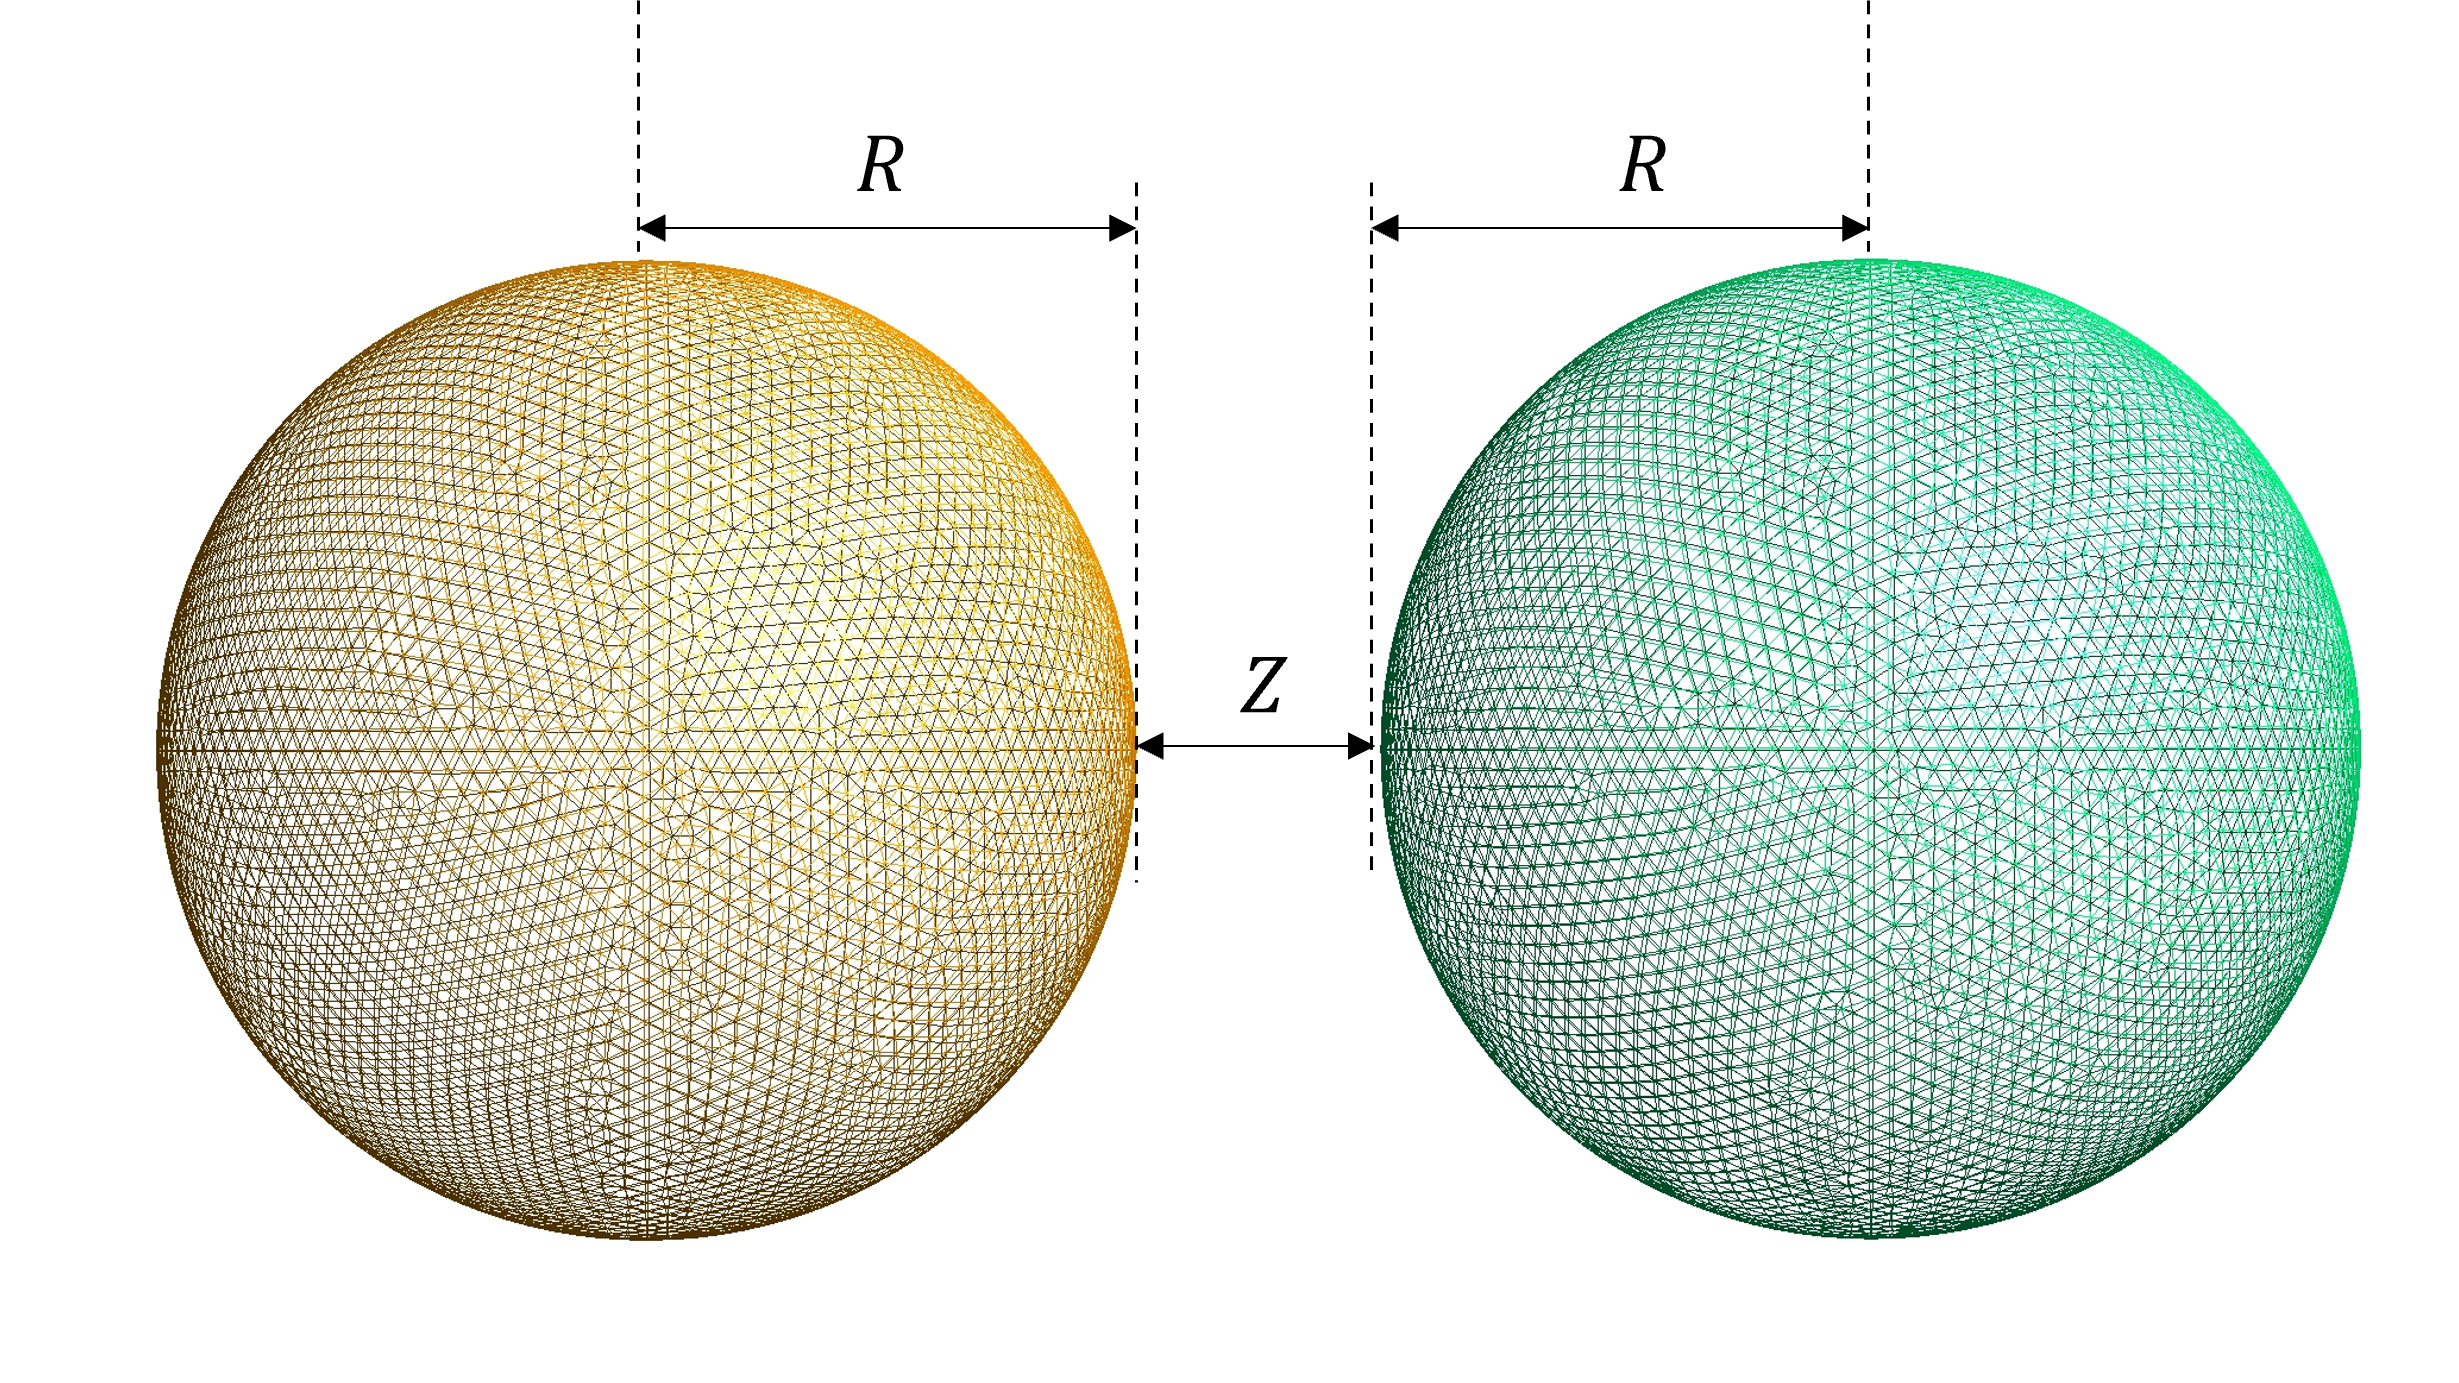
\includegraphics[scale = 0.6]{figures/Grid_two_spheres_dist.png}
    \caption{Two spheres with equal radii: $R$ represents the radius of the spheres and $Z$ is the distance between them.}
    \label{Two spheres with equal radii}
\end{figure}

\begin{figure}[H]
    \includegraphics[scale = 0.7]{figures/rel_dist_equal_radii.pdf}
    \caption{Relative distance between the reference value (computed by Richardson extrapolation) with the asymptotic series, the estimates evaluated when the 
    grid size $h = 0.05$ and 0.1, the estimates evaluated by the standard Arnoldi method and inverse-free Krylov subspace method.
     {\color{red}{should add inverse-free Krylov method later on the figure}}}
    \label{equal_radii_rel_dist}
\end{figure}

From the Figure \ref{equal_radii_rel_dist}, when the grid size $h$ decreases from 0.1 to 0.05, the relative distance between the exact value of the Casimir energy and the estimates 
goes down as well. Since the asymptotic expansion of the Casimir energy only works when the distance between two spheres is asymptotically large, the relative 
distance between the exact value and the asymptotic one decreases as we increase the distance between the spheres. In addition, we apply the standard Arnoldi
method to efficiently compute the Casimir energy and set the dimension of the Krylov subspace inside the algorithm as $m = 20$ and $50$ and we can easily find 
as we increase the Krylov subspace dimension, the relative distance decreases.

\begin{figure}[H]
    \hspace*{2cm}\includegraphics[scale = 0.6]{figures/Grid_two_spheres_unequal_radii.png}
    \caption{Two spheres with unequal radii: $R_{1}$ and $R_{2}$ represent the radius of the spheres and $Z$ is the distance between them.}
    \label{Two spheres with unequal radii}
\end{figure}

When the perfectly conducting spheres have different radii (see Figure \ref{Two spheres with unequal radii}), $R_{1}$ and $R_{2}$ and the centre distance 
is $L = 2R+Z$, then the asymptotic expansion of the Casimir energy at asymptotically large distance can be written as:
\begin{align}\label{Asymptotic unequal radii}
    \mathcal{E} = -\frac{\hbar c}{\pi}\frac{1}{L}\sum_{n=0}^{\infty}\tilde{b}_{n}(\eta)\left(\frac{R_{1}}{L}\right)^{n+2},
\end{align}
where the coefficients $\{\tilde{b}_{n}\}$ depend on the parameter $\eta = R_{2}/R_{1}$ and the first six coefficients are
\begin{align*}
    \tilde{b}_{0} &= -\frac{\eta}{4}, \ \ \ \ \ \tilde{b}_{1} = -\frac{\eta + \eta^{2}}{8}, \ \ \ \ \  \tilde{b}_{2} = -\frac{34(\eta+\eta^{3})+ 9\eta^{2}}{48}, \ \ \ \ \ \tilde{b}_{3} = -\frac{2(\eta+\eta^{4}) + 23(\eta^{2} + \eta^{3})}{32}, \\ 
    \tilde{b}_{4} &= -\frac{8352(\eta + \eta^{5})+ 1995(\eta^{2} + \eta^{4}) + 38980\eta^{3}}{5760}, \ \ \ \ \ \tilde{b}_{5} = -\frac{-1344(\eta+\eta^{6}) + 5478(\eta^{2} + \eta^{5})+2357(\eta^{3} + \eta^{4})}{2304}.
\end{align*}
({\color {red}{Add relative distance figure for unequal radii case }} )

\subsection{Realistic objects case}
{\color {blue} The scatterers are set as some realistic objects (or something complex such as 8-branch ice crystal) and we compute the Casimir energy between them 
in the scalar case.} 
